\subsection{Function discriminant analysis, FDA}

\begin{figure}[h]
\begin{center}
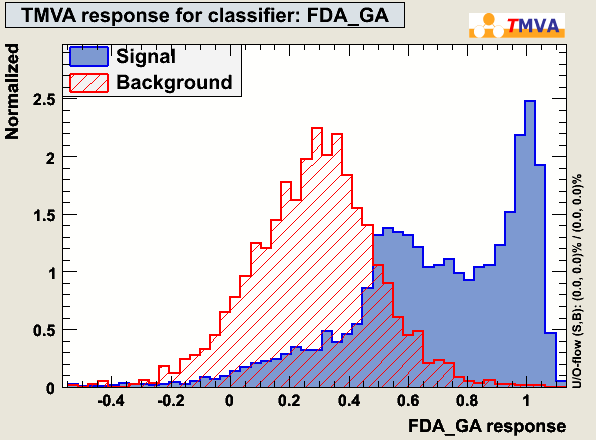
\includegraphics[width=1.0\textwidth]{images/pkMva_FDA_GA.png}
\caption{mvaFDA using genetic algorighm (GA)}
\label{fig:pkMvaFDAGA}
\end{center}
\end{figure}

\begin{figure}[h]
\begin{center}
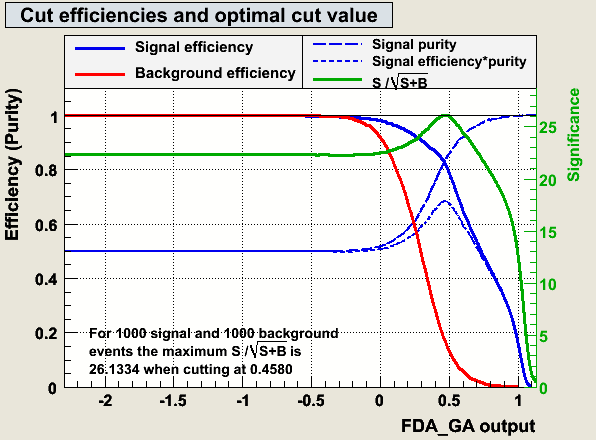
\includegraphics[width=1.0\textwidth]{images/pkMvaEffs_FDA_GA.png}
\caption{FDA GA }
\label{fig:pkMvaEffsFDAGA}
\end{center}
\end{figure}

\begin{figure}[h]
\begin{center}
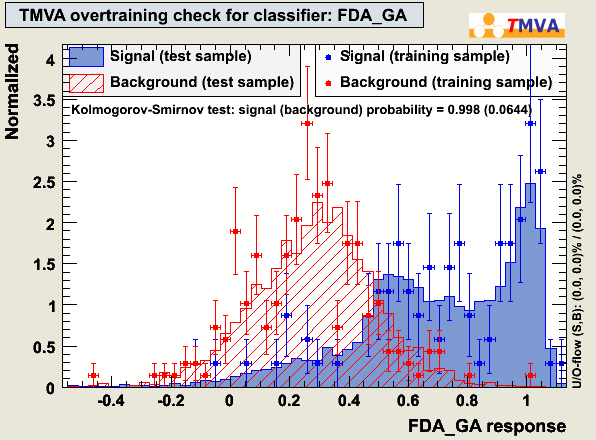
\includegraphics[width=1.0\textwidth]{images/pkOvertrain_FDA_GA.png}
\caption{FDA GA }
\label{fig:pkOvertrainFDAGA}
\end{center}
\end{figure}


\subsection{k-nearest neighbour method, kNN}

\begin{figure}[h]
\begin{center}
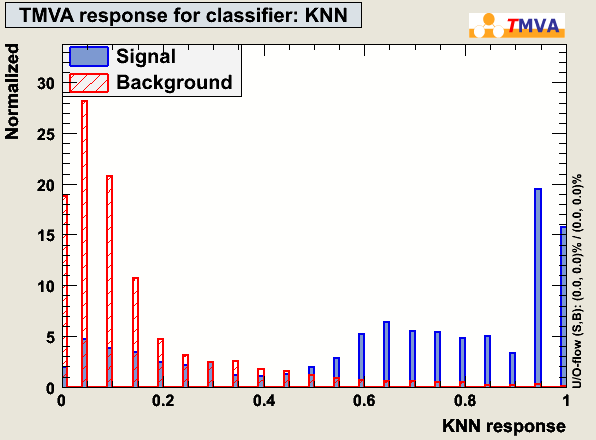
\includegraphics[width=1.0\textwidth]{images/pkMva_KNN.png}
\caption{MVAKNN}
\label{fig:pkMvaKNN}
\end{center}
\end{figure}

\begin{figure}[h]
\begin{center}
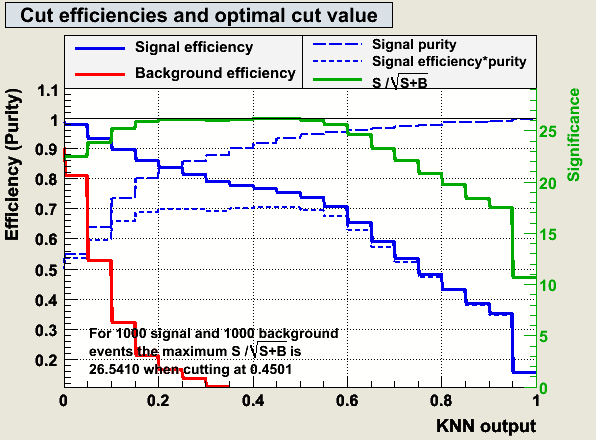
\includegraphics[width=1.0\textwidth]{images/pkMvaEffs_KNN.png}
\caption{KNN}
\label{fig:pkMvaEffsKNN}
\end{center}
\end{figure}

\begin{figure}[h]
\begin{center}
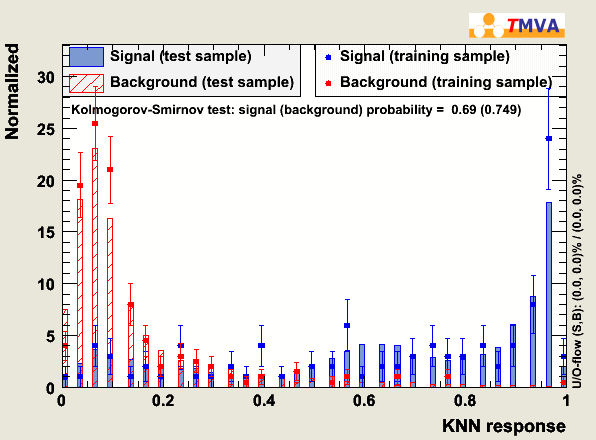
\includegraphics[width=1.0\textwidth]{images/pkOvertrain_KNN.png}
\caption{KNN}
\label{fig:pkOvertrainKNN}
\end{center}
\end{figure}

\begin{figure}[h]
\begin{center}
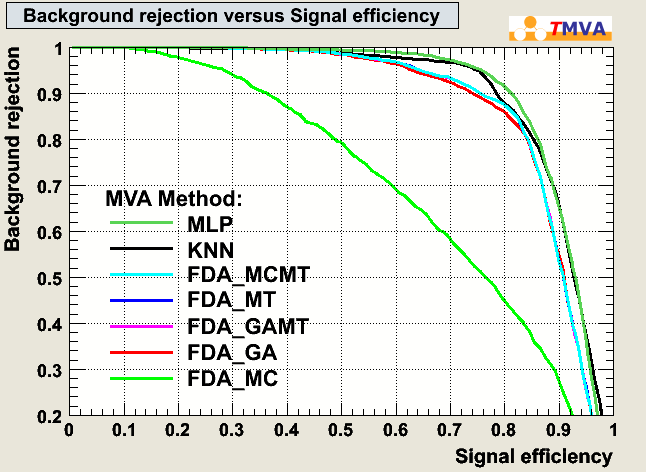
\includegraphics[width=1.0\textwidth]{images/pkRejBvsS.png}
\caption{ROC curve (MLP added as a benchmark)}
\label{fig:pkRejBvsS}
\end{center}
\end{figure}

\clearpage
